%% ****** Start of file apstemplate.tex ****** %
%%
%% This file is part of the APS files in the REVTeX 4 distribution.
%% Version 4.1r of REVTeX, August 2010
%%
%%
%% Copyright (c) 2001, 2009, 2010 The American Physical Society.
%%
%% See the REVTeX 4 README file for restrictions and more information.
%%
%
% This is a template for producing manuscripts for use with REVTEX 4.0
% Copy this file to another name and then work on that file.
% That way, you always have this original template file to use.
%
% Group addresses by affiliation; use superscriptaddress for long
% author lists, or if there are many overlapping affiliations.
% For Phys. Rev. appearance, change preprint to twocolumn.
% Choose pra, prb, prc, prd, pre, prl, prstab, prstper, or rmp for journal
%  Add 'draft' option to mark overfull boxes with black boxes
%  Add 'showpacs' option to make PACS codes appear
%  Add 'showkeys' option to make keywords appear
\documentclass[aps,pra,reprint,longbibliography,groupedaddress]{revtex4-1}
%\documentclass[aps,prl,preprint,superscriptaddress]{revtex4-1}
%\documentclass[aps,prl,reprint,groupedaddress]{revtex4-1}

% You should use BibTeX and apsrev.bst for references
% Choosing a journal automatically selects the correct APS
% BibTeX style file (bst file), so only uncomment the line
% below if necessary.
%\bibliographystyle{apsrev4-1}
\usepackage{graphicx}
\usepackage{amssymb, amsmath}
\usepackage{esdiff} % use this package for derivative and partial derivate commands of \diff{}{} and \diffp{}{}
\usepackage{siunitx}
\usepackage{multirow}
\usepackage{verbatim}
\usepackage{newfloat}
\usepackage{afterpage} 
\usepackage{xr}
\DeclareSIUnit\cells{cells}
\DeclareMathOperator{\hilbert}{\mathcal{H}} % To define additional named operators
\DeclareMathOperator{\h}{h} % To define additional named operators
\DeclareMathOperator{\unwrap}{unwrap} % To define additional named operators
\DeclareMathOperator{\vercat}{cat_\downarrow} % To define additional named operators
\DeclareMathOperator{\horcat}{cat_\rightarrow} % To define additional named operators
\DeclareFloatingEnvironment[name={Supplementary Figure}]{suppfigure}
\renewcommand{\thefigure}{S\arabic{figure}}
\renewcommand{\thetable}{S\arabic{table}}
\externaldocument[M-]{main}



\begin{document}
%Title of paper
\title{Deep learning for high-throughput label-free cell classification}

% repeat the \author .. \affiliation  etc. as needed
% \email, \thanks, \homepage, \altaffiliation all apply to the current
% author. Explanatory text should go in the []'s, actual e-mail
% address or url should go in the {}'s for \email and \homepage.
% Please use the appropriate macro foreach each type of information

% \affiliation command applies to all authors since the last
% \affiliation command. The \affiliation command should follow the
% other information
% \affiliation can be followed by \email, \homepage, \thanks as well.
\author{Claire L. Chen}
%\homepage[]{Your web page}
%\thanks{}
\author{Ata Mahjoubfar}
\author{Li-Chia Tai}
\author{Ian K. Blaby}
\author{Allen Huang}
\author{Kayvan R. Niazi}
\author{Bahram Jalali}

%Collaboration name if desired (requires use of superscriptaddress
%option in \documentclass). \noaffiliation is required (may also be
%used with the \author command).
%\collaboration can be followed by \email, \homepage, \thanks as well.
%\collaboration{}
%\noaffiliation

\date{\today}
% insert suggested PACS numbers in braces on next line
%\pacs{}
% insert suggested keywords - APS authors don't need to do this

%\maketitle must follow title, authors, abstract, \pacs, and \keywords
\maketitle

% body of paper here - Use proper section commands
% References should be done using the \cite, \ref, and \label commands
\section*{Supplementary methods}

\begin{figure*}
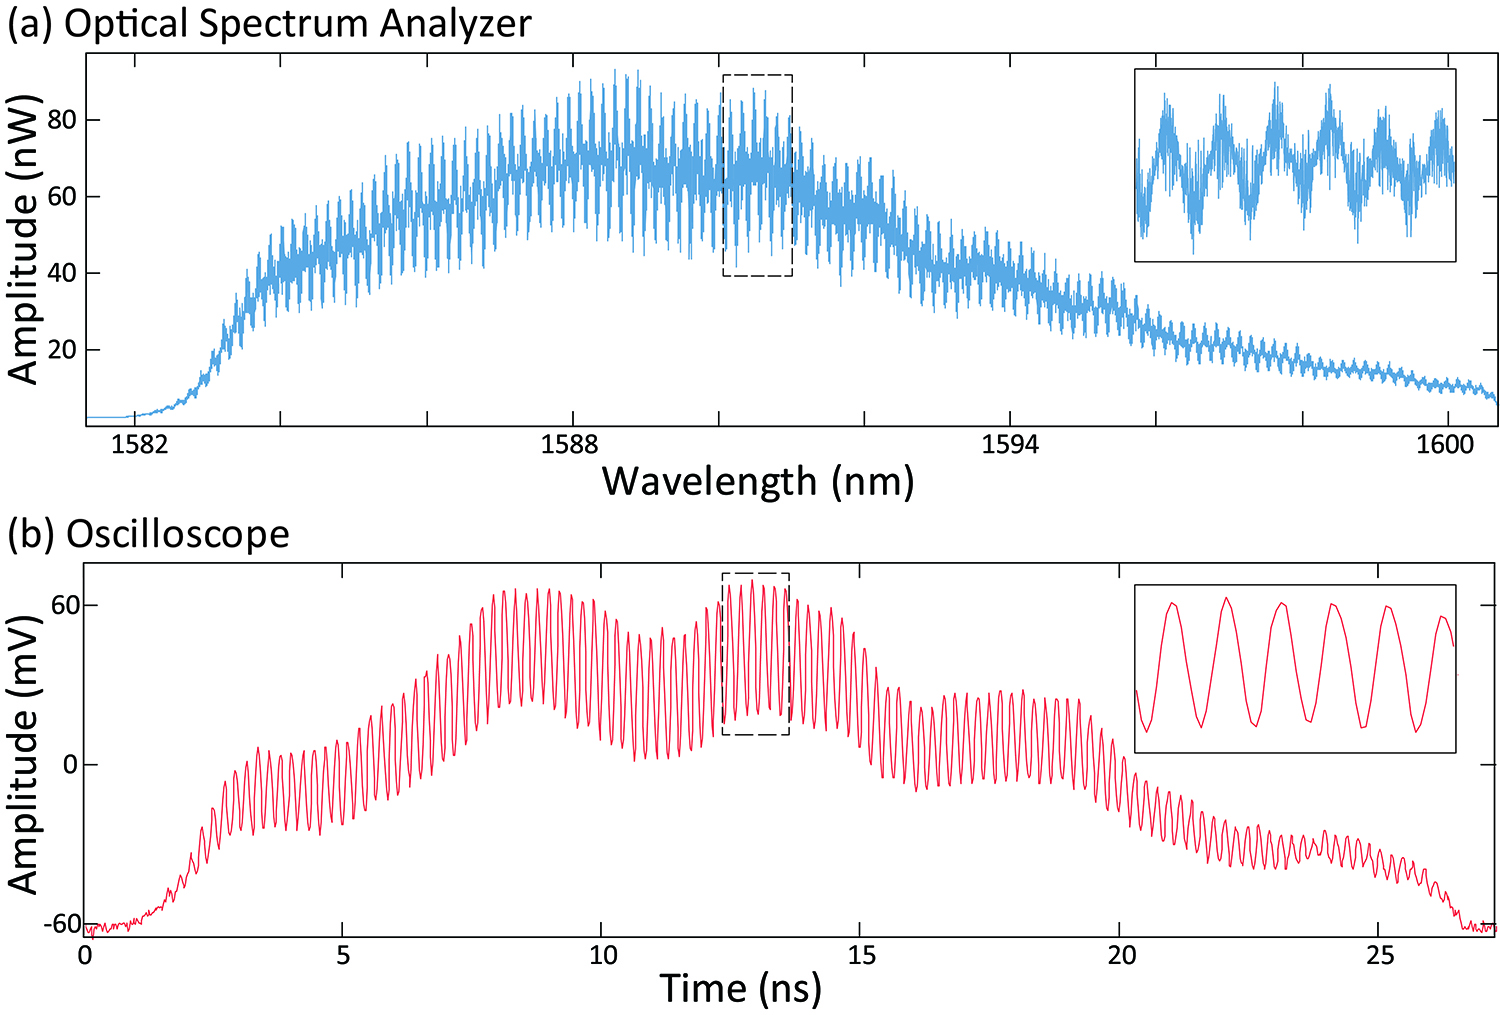
\includegraphics[scale=0.5]{FigureOSA.jpg}
\caption{\label{fig:OSA} Comparison of the interferograms measured by optical spectrum analyzer and time-stretch dispersive Fourier Transform; (a) Optical spectrum of the signal after quantitative phase imaging (box 1 in Fig.~\ref{M-fig:Setup}) and before it enters the amplified time-stretch system (box 2 in Fig.~\ref{M-fig:Setup}). The interference pattern in spectral domain is measured by an optical spectrum analyzer. (b) With time stretch, the interference pattern in spectral domain is linearly mapped into time. The baseband intensity envelope is slightly modified by the wavelength-dependent gain profile of the Raman amplifier. The inserts in panels a and b show the zoomed-in spectrum and waveform in the dashed black boxes, respectively. Clearly, the single-shot interferogram measured by Raman-amplified time-stretch dispersive Fourier Transform has a higher signal-to-noise ratio compared to that captured by optical spectrum analyzer.}
\end{figure*}

\section{Principal component analysis (PCA)}

As shown in Fig.~\ref{M-fig:FeaturesCorrRank}a and Fig.~\ref{M-fig:FeaturesCorrRank}b, many of the 16 features are correlated and not all measured features in the data set produced by the time stretch quantitative phase imaging have the same amount of information. That result suggests that it may be possible to reduce the 16 dimensional data set to a smaller set of uncorrelated orthogonal dimensions without significantly compromising the classification accuracy. In that spirit, we have used principle component analysis (PCA) for dimensionality reduction and computation speed-up. The PCA algorithm finds an alternative lower dimension space such that variance of data projected onto this subspace is maximized along subspace dimensions. Fig.~\ref{fig:PCA}a shows the percent of the variance in data explained by each component (lower chart). The key observation is that most of the variance can be accounted for by the first two principle components. The upper portion of the plot shows the accuracy for binary classification using each of the principle components. Interestingly, the first component with the highest explained variance is not necessarily the most important component for classification. Therefore, apriori intuition about the physical significance of the features in the case here, is superior to PCA in eliminating dimensions that do not provide high value in classification. By revealing the structure in data that best explains the variance, PCA achieves data compression via dimensionality reduction. 

PCA components acts as the input features for the classification algorithm. As number of PCA components retained increases, the classification accuracy improves while computation time increases (Fig.~\ref{fig:PCA}b). Since accuracy is the main concern here, we employ all 16 biophyscial features, rather than dimensionality-reduced PCA compoents.

\begin{figure*}
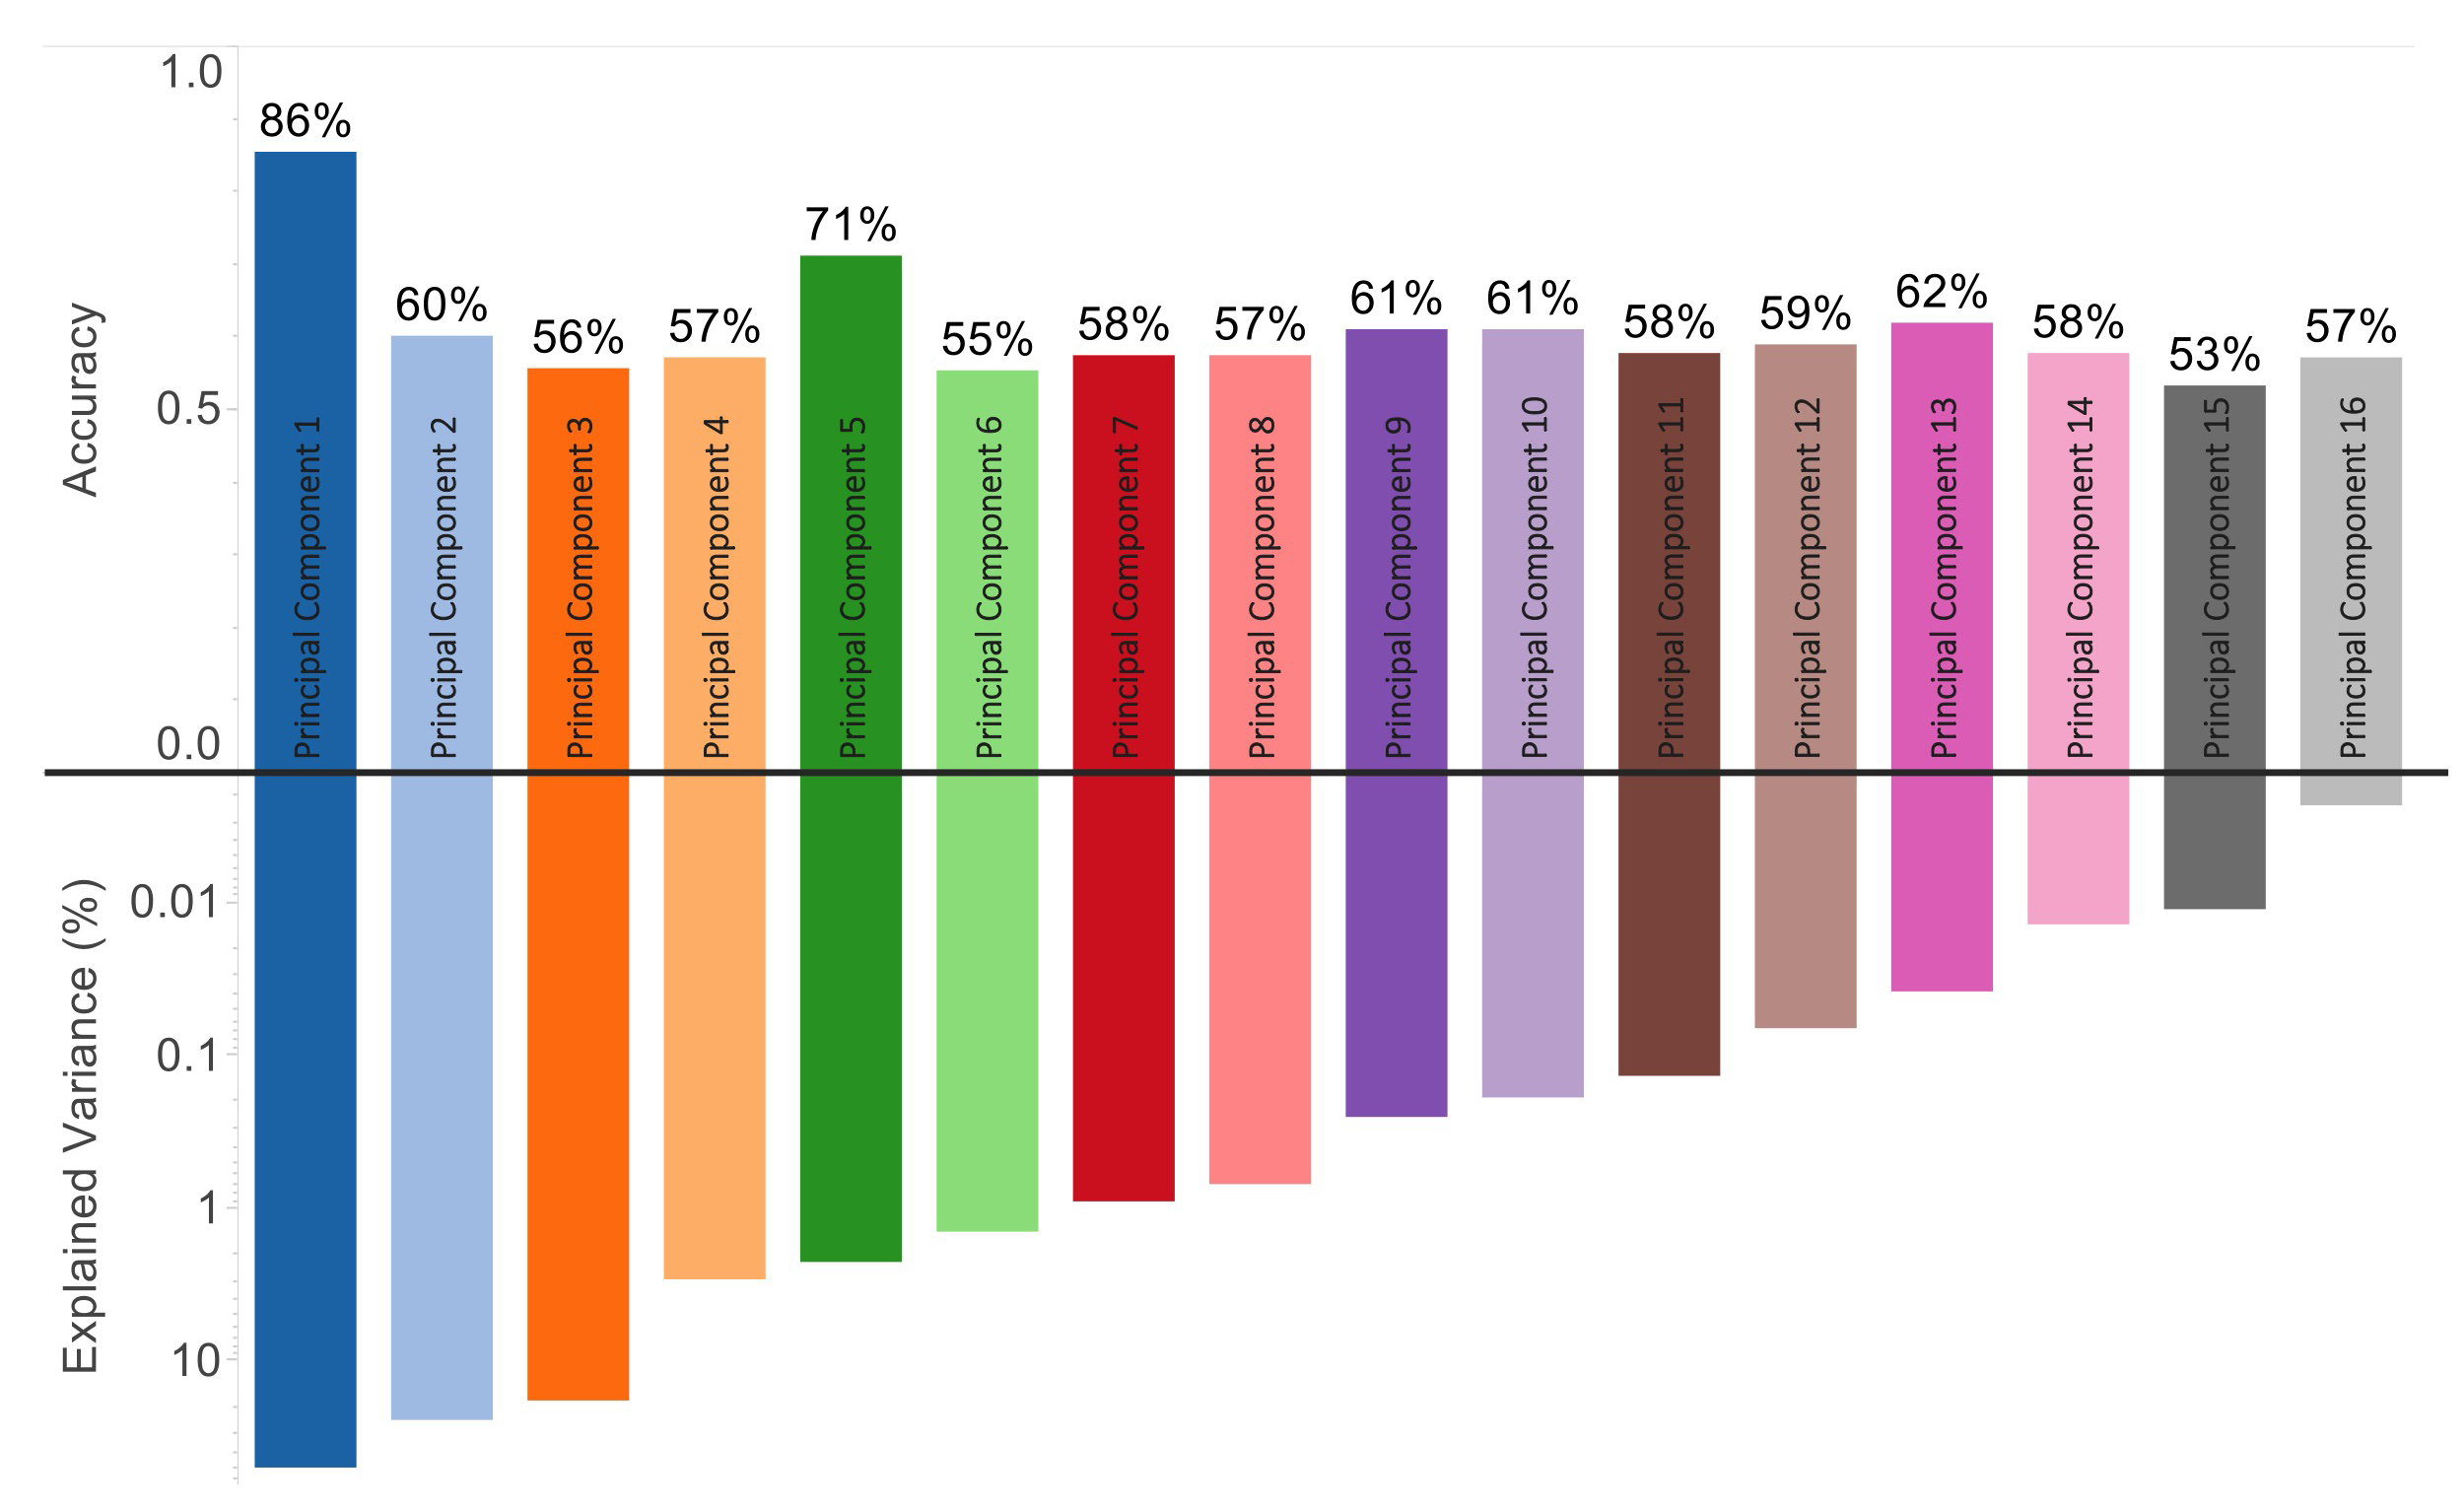
\includegraphics[scale=0.18]{FigurePCA.jpg}
\caption{\label{fig:PCA} 
Principal component analysis (PCA) on the multivariate data set produed by time stretch quantitative phase imaging. (a) Upper bar chart shows accuracy of classification by each individual principal component, and lower bar chart shows the percentage of the total variance explained by each principal component, accounting for the variability expressed in the data. As expected, principal components with larger variability do not necessarily give high accuracy in classification. (b) In order to reduce the number of input features and decrease computation time, a subset of the PCA components are used for classification. The classification accuracy improves as the the total variance retained in the subset of PCA components goes up.}
\end{figure*}

\section{\label{scn:CrossValidation}Cross validation} 

The k-fold cross-validation implemented here splits data points into training, validation, and test subsets (Fig.~\ref{fig:CrossVaidationRegularization}a). For each interation, one fold is used as test data, one for validation while the other folds are used during training process. After innitially trained, the performance of the network is analyzed by the validation data to fine tune the neural network architecture and regularization parameter. Fig.~\ref{fig:CrossVaidationRegularization}b shows that either a too small or a too large regularization parameter, $\lambda$, increases network error due to overfitting or underfitting, respectively. Therefore, there is a suitable range of regularization parameter for each learning model.

Once the network architecture and regularization parameter are chosen and optimized based on the validation data, the learning model performance is finally verified by the test fold, which has never been used before in this interation. The process of training in each iterations is independent, so each iteration has no prior knowledge about the chosen learning models in other iterations. The final reported results are aggregate of the performance for different test datasets.

\begin{figure*}
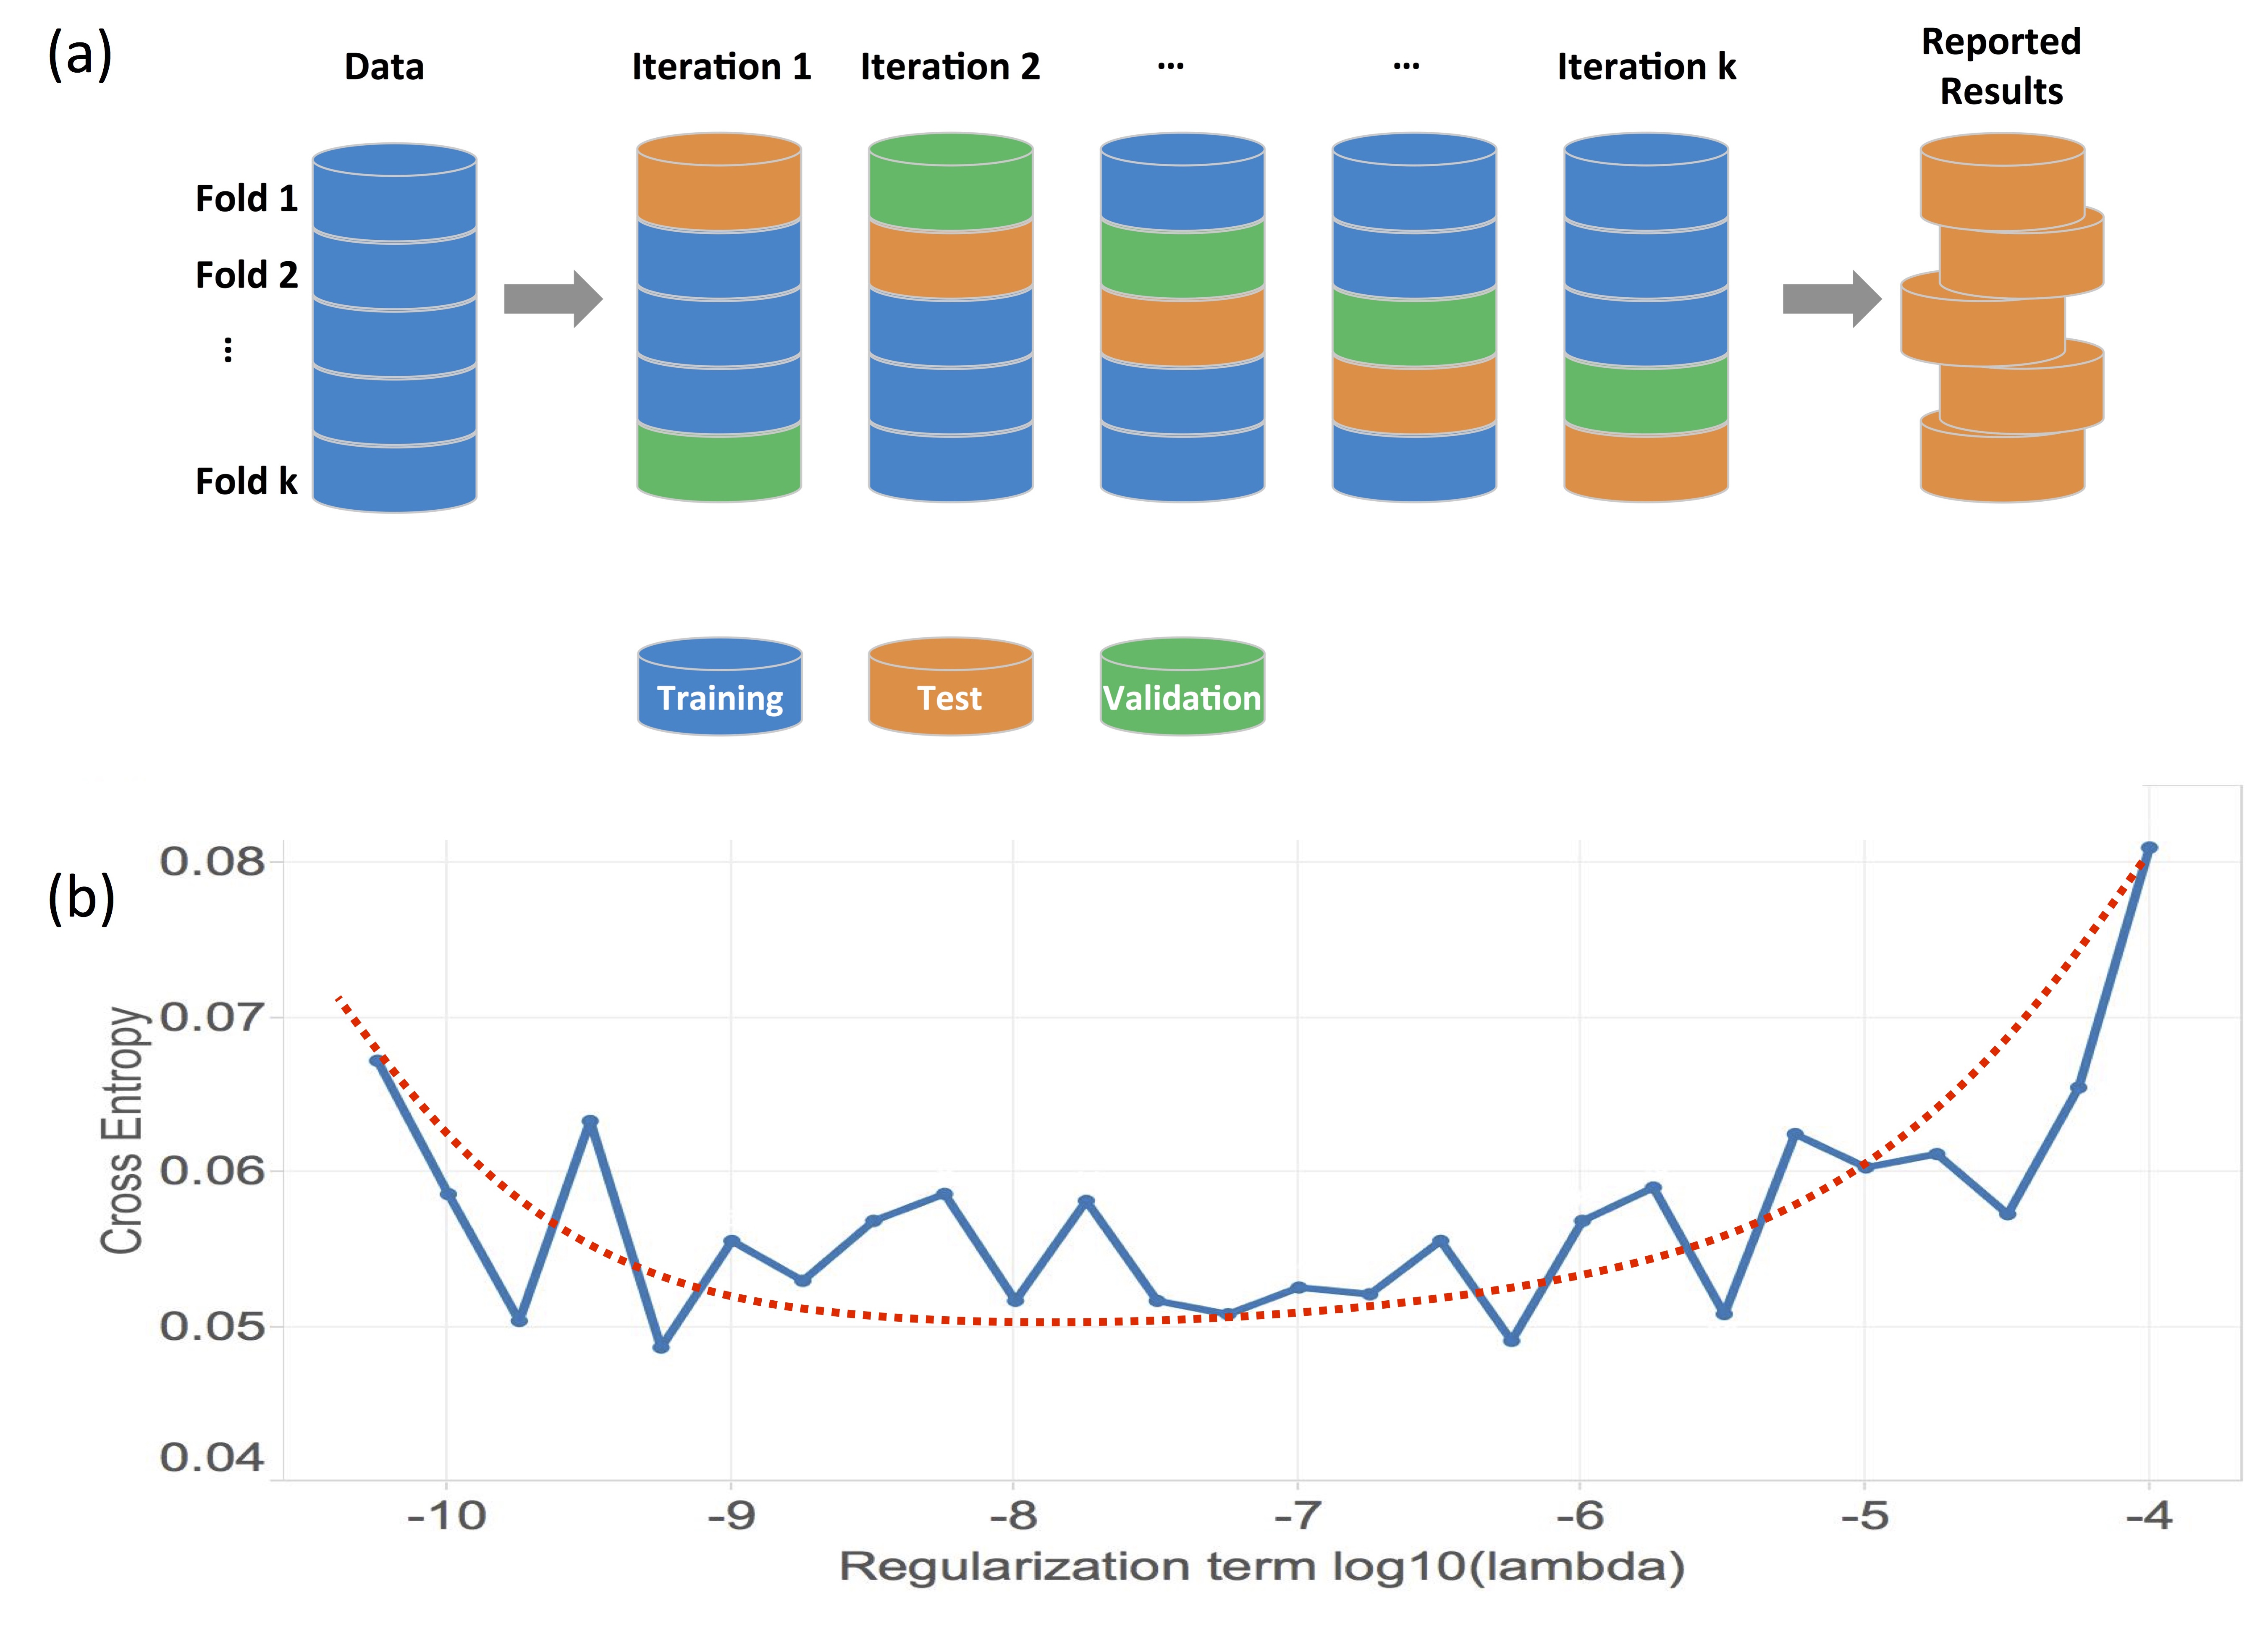
\includegraphics[scale=0.08]{FigureCrossValidationRegularization.jpg}
\caption{\label{fig:CrossValidationRegularization} 
(a) The implementation of the k-fold cross-validation here splits data points into training, validation, and test subsets. In each iteration, one fold is used for fine tuning the learning model (validation dataset) and another fold is used for evaluation of the final results (test dataset), while rest of the data points are used for training (training dataset). The final reported results are aggregate of the outcomes from the test datasets. (b) A suitable regularization parameter, $\lambda$, balances the trade-off between overfitting (variance) and underfitting (bias) and minimizes the cross entropy of the validation dataset.}
\end{figure*}

\section{System performance and resolvable points}

Lateral resolution of time stretch camera is decided by the limiting factor among Abbe diffraction limit of the objective lens, spectral resolvability of the diffraction grating pairs, spectral resolution in amplified dispersive Fourier transform, the photodetector rise-time and bandwidth, and the sampling rate of the back-end digitizer. Details of the limiting factors of lateral resolution and evaluation of these factors for our TS-QPI system can be found in Table~\ref{tbl:Resolution}. Field of view (FOV) is the area covered by the interrogation rainbow when the rainbow pulses hit the imaging plane. The rainbow pulse width is decided by the optical bandwidth selected from the laser source, $\Delta\lambda$, the magnification factor of the objective lens, the focal length of the other lenses and parabolic mirrors, as well as the dimensions and blaze angles of the diffraction gratings.

\begin{table*}
\caption{\label{tbl:Resolution} Resolution Limiting Factors in TS-QPI}
\begin{tabular}{|m{0.16\textwidth}|m{0.15\textwidth}|m{0.45\textwidth}|m{0.10\textwidth}|}
 \hline
 System catagory   &Component  &Number of resolvable points &Lateral resolution    \\  \hline
\multicolumn{1}{ |m{0.16\textwidth}  }{\multirow{2}{*}{Free-space optics} } &
\multicolumn{1}{ |m{0.15\textwidth}| }{Diffraction gratings} & \begin{equation} N_{grating} = \frac{\Delta\lambda}{\delta\lambda_{grating}} =\Delta\lambda /(\lambda \cdot \frac{d}{m\cdot2w_0})\end{equation} where $\Delta\lambda$ is the optical bandwidth, $\lambda$ is the central wavelength, m is the order of diffraction, $w_0$ is the beam waist, and $d$ is the groove spacing. &$\SI{3.09}{\micro\meter}$ \\ \cline{2-4}
\multicolumn{1}{ |m{0.15\textwidth}  }{}         &
\multicolumn{1}{ |m{0.15\textwidth}| }{Lenses and mirrors} & \begin{equation} N_{Abbe} = \frac{FOV}{\delta x_{diffraction}} =\frac{FOV}{(\frac{\lambda + \Delta \lambda/2}{2 \cdot NA})} \end{equation} where $FOV$ is field of view, $NA$ is numerical aperture of the objective lens. &$\SI{2.00}{\micro\meter}$   \\ \cline{1-4}
\multicolumn{1}{ |m{0.16\textwidth}  }{\multirow{1}{*}{Time Stretch} } &
\multicolumn{1}{ |m{0.15\textwidth}| }{Group delay dispersion} &\begin{equation}N_{DFT}=\frac{\Delta\lambda}{\delta\lambda}=\frac{\Delta\lambda}{\lambda\cdot\sqrt{\frac{2}{DL_f\cdot c}}}\end{equation} where $D$ is the group velocity dispersion, $L_f$ is the dispersive fiber length. &$\SI{0.73}{\micro\meter}$ \\ \cline{1-4}
\multicolumn{1}{ |m{0.16\textwidth}  }{\multirow{2}{*}{Electronic back-end} } &
\multicolumn{1}{ |m{0.15\textwidth}| }{Photodetector bandwidth} &\begin{equation}N_{PD}=\frac{\Delta t}{\delta t}=\frac{DL_f\Delta\lambda}{0.35/B}\end{equation} where $B$ is the bandwidth of the photodetector. &$\SI{0.28}{\micro\meter}$ \\ \cline{2-4}
\multicolumn{1}{ |m{0.15\textwidth}  }{} &
\multicolumn{1}{ |m{0.15\textwidth}| }{ADC sampling rate} &\begin{equation}N_{ADC}=DL_f\Delta\lambda f_{ADC}\end{equation} where $f_{ADC}$ is the sampling rate of digitizer. &$\SI{0.10}{\micro\meter}$ \\
\cline{1-4}
\end{tabular}
\end{table*}

The resolution of phase measurement along axial direction is determined by the effective number of bits (ENOB) of the digitizer and affected by the noise of laser source. Since pulse-to-pulse intensity and phase fluctuations are small, noise from laser source is not the limiting factor in our phase measurements. Supposing the ENOB of the digitizer is $N$, the minimum detectable optical path length difference, $\Delta L$ can be estimated as
\begin{equation}
\frac{1}{2}sin\left(\frac{4\pi \Delta L}{\lambda + \Delta \lambda/2}\right)=2^{-N}
\end{equation}
where $\lambda$ is the central wavelength of light, and $\Delta\lambda$ is the optical bandwidth. In our system, ENOB of the analog-to-digital converter is $5$. Thus, the OPD resolution along the axial direction is about $\SI{8.0}{\nano\meter}$, corresponding to refractive index difference down to the order of $0.001$ for cellular level measurements.

\section{Microfluidic channel design and fabrication}

The Polydimethylsiloxane (PDMS) microfluidic channel is custom-designed so that it could fit into the reflective optics design. Cells are hydrodynamically focused \cite{knight1998hydrodynamic,lee2006hydrodynamic} at the center of the channel flowing at a velocity of 1.3 m/s. The microfluidic device consists of a hydrodynamic focusing region and an imaging region targeted by the interrogation rainbow flashes in TS-QPI system. At the hydrodynamic focusing region, the sheath pressure focused the sample at the center of the channel by narrowing its flow width from \SI{200}{\micro\meter} to about \SI{40}{\micro\meter} with a sheath to sample volume ratio of 3:1. The dimension of the channel was chosen as \SI{200}{\micro\meter} (width) $\times$ \SI{25}{\micro\meter} (height) so that the cells will be imaged within depth of focus with a narrow lateral distribution. The size of the entire PDMS channel is optimized for fitting on a 2 inch diameter dielectric mirror with sufficient space at the edges to achieve strong bonding. The thickness of the channel top layer is optimized for stabilizing peek tubes performance reliability while accommodating the working distance of the objective lens. 

\begin{figure}
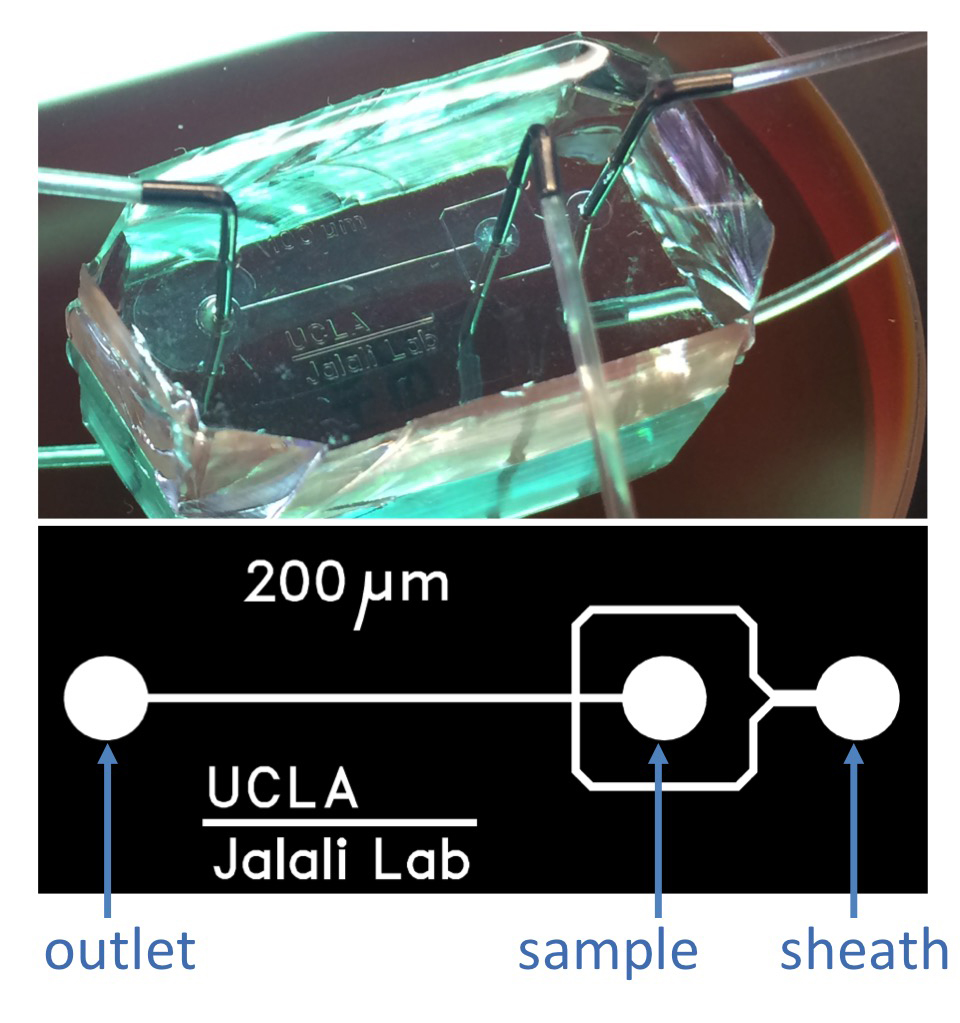
\includegraphics[scale=0.2]{FigureChannel.jpg}
\caption{\label{fig:Channel} PDMS microfluidic channel mounted on a highly reflective surface with near-infrared dielectric coating; The microfluidic device consists of a hydrodynamic focusing region and an imaging region targeted by the interrogation rainbow flashes in TS-QPI system. (a) Sample solution with suspended cells is fed into the channel through the sample inlet, and deionized water as the sheath fluid is injected through the sheath inlet. At the hydrodynamic focusing region, the sheath pressure focused the sample at the center of the channel by narrowing its flow width from \SI{200}{\micro\meter} to about \SI{40}{\micro\meter} with a sheath to sample volume ratio of 3:1. (b) The pattern of the mask used to imprint microfluidic channel design on silicon wafer with photoresist. The circles are inlet and outlet reservoirs.}
\end{figure}

The PDMS microfluidic channel (Fig.~\ref{fig:Channel}) is fabricated using standard soft lithography. The mask was designed in AutoCAD and printed with a resolution down to \SI{1}{\micro\meter}. Then a 4-inch silicon wafer was spin-coated with \SI{75}{\micro\meter} thickness of a negative photoresist (SU-8 from MicroChem) and was exposured under the mask using an aligner. After post-exposure baking, the wafer was developed at room temperature, rinsed with isopropyl alcohol (IPA), and placed in a petri dish. A PDMS mixture (Sylgard 184 Silicone Elastomer, Dow Corning) was poured onto the patterned wafer, degassed in a vacuum chamber for 30 min and cured at \SI{80}{\degreeCelsius} for one hour. Once cured, the PDMS channel was cut out and peeled off from the master wafer. We used \SI{1.25}{\micro\meter} diameter hollow needle to punch the inlet and outlet holes. 
The punched PDMS channel was then cleaned with nitrogen gun and magic tape (3M), treated with oxygen plasma (Enercon Dyne-A-Mite 3D Treater) for 2 min, and bonded to a 2-inch diameter broadband dielectric mirror (Thorlabs BB2-E04) for obtaining high reflectance from channel substrate at near infrared spectral window. Finally microtubes (PE-50 tubing, $.023 \times .038$ in) with steel catheter couplers (Instech, 22 ga $\times 15$ mm) are connected to the inlet and outlet punctures.


\section{Preparation of algae cell lines}

\textit{Chlamydomonas reinhardtii} strains used were \textit{cw15} (\textit{nit1 NIT2 mt$^{+-}$}) and \textit{sta6} (\textit{cw15 nit1 NIT2 arg7-7 sta6-1::ARG7 mt$^+$}), available as CC-4568, CC-4348 respectively from the Chlamydomonas resource center (CRC)\cite{minnesota2015chlamydomonas}.

Cells were grown in tris-acetate-phosphate (TAP) medium supplemented with arginine (\SI{100}{\micro\gram\per\milli\liter}). Cultures were grown in Innova incubators (New Brunswick Scientific, Edison, NJ) at \SI{24}{\degreeCelsius}, agitated at 180 rpm with continuous light (\SI{95}{\micro\mole\per\square\meter\per\second}, 6 cool white fluorescent bulbs at \SI{4100}{\kelvin} and 3 warm white fluorescent bulbs at \SI{3000}{\kelvin} per incubator). To induce lipid production, cells were cultured to mid-log phase in regular TAP prior to deprivation of N by transfer to ammonium-free (i.e. nitrogen-free) TAP medium, as described previously \cite{blaby2013systems}. Briefly, cells subjected to nitrogen deprivation were grown to \SI{4e6}{\cells\per\milli\liter} and collected by centrifugation at 1006 xg for 5 min at room temperature. The supernatant was discarded, and the cells were washed in nitrogen-free TAP. Cells were then resuspended in nitrogen-free TAP to a final cell count of \SI{2e6}{\cells\per\milli\liter}. Cell densities were determined using a hemocytometer.


% Create the reference section using BibTeX:
%merlin.mbs apsrev4-1.bst 2010-07-25 4.21a (PWD, AO, DPC) hacked
%Control: key (0)
%Control: author (0) dotless jnrlst
%Control: editor formatted (1) identically to author
%Control: production of article title (0) allowed
%Control: page (1) range
%Control: year (0) verbatim
%Control: production of eprint (0) enabled
\bibliography{main}



\end{document}
%
% ****** End of file apstemplate.tex ******

